Este capítulo é dedicado à introdução do leitor ao principal tópico de estudo do projeto e assim mostrar
algumas aplicações onde este é usado, além de apresentar os desafios relacionados à estas aplicações.

\section{Resposta ao Impulso de Ambiente Acústico e suas Aplicações}

Dentre os diversos tópicos na grande área de estudo de sinais de áudio, destaca-se a detecção e reconhecimento de fontes acústicas no espaço físico.
Um caso específico deste tópico é sobre sinais de voz gravados em ambientes fechados, onde um ou mais microfones são posicionados na sala afastados
da fonte sonora, normalmente uma pessoa que performa a gravação.
Estes sinais são corrompidos pela reverberação do ambiente, que surge a partir da sobreposição da onda sonora anecoica que chega ao microfone com a 
onda sonora atenuada e refletida nas paredes do ambiente fechado. 

\begin{figure} [H]
    \begin{subfigure}{.5\textwidth}
        \centering
        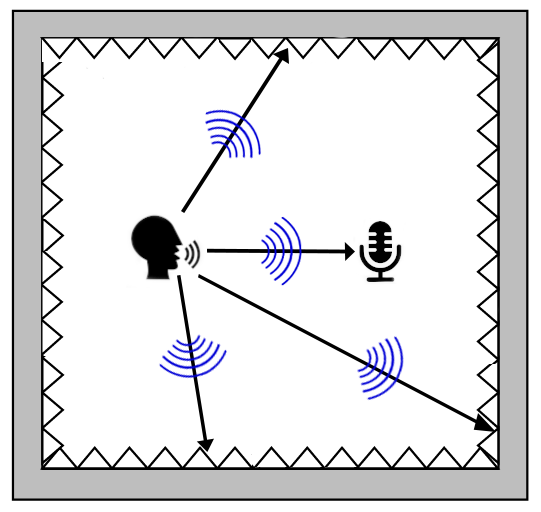
\includegraphics[scale=0.4]{camara_anecoica.png}
        \caption{Sala anecoica}    
    \end{subfigure}
    \begin{subfigure}{.5\textwidth}
        \centering
        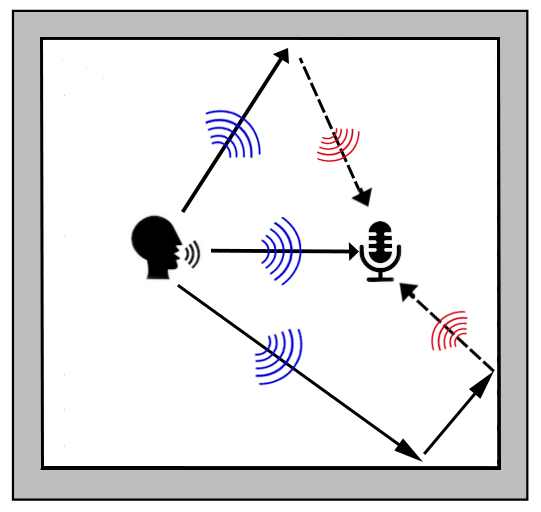
\includegraphics[scale=0.4]{camara_reverb.png}    
        \caption{Sala reverberante}    
    \end{subfigure}
    \caption{Representação de uma sala anecoica e reverberante}
    \label{fig:Rooms}
\end{figure}

Observa-se na figura \ref{fig:Rooms} uma representação de uma sala anecoica, onde o único áudio capturado pelo microfone é a onda sonora direta
enviada pela fonte, sem nenhuma reflexão do ambiente; já na sala reverberante, nota-se que o áudio capturado será uma combinação da onda sonora direta
com as refletidas nas paredes. 
Este sinal reverberado pode ser modelado da seguinte forma:

\begin{equation} \label{eqn:model}
    Y(t) = s(t) \ast h(t) + n(t)
\end{equation}

% ### TODO: [FIGURA] exemplificando voz reverberada e figura mostrando o que é RIR

Onde $Y(t)$ representa o sinal de voz em campo distante, $s(t)$ o sinal de voz anecoico, $h(t)$ a RIR e $n(t)$ o sinal de ruído que pode
estar presente no ambiente.
Dessa forma, é possível inferir que a RIR representa o modelo acústico de uma sala, para uma determinada combinação de fatores do ambiente, incluindo: 
temperatura e umidade relativa do ar, pressão atmosférica, material das paredes e posicionamento de móveis.
Reverberação causa degradação do sinal de voz, levando à perda de clareza na comunicação \cite{Speech_intellig_hear} e à redução da performance
de sistemas de reconhecimento de voz \cite{reverb_sup_speech_reg}. Este problema demonstra a necessidade de identificar dinamicamente o modelo acústico
do ambiente para que possam ser mitigadas as perdas nas amostras de voz gravadas e assim facilitar os algoritmos que usam esses sinais.

Este projeto é focado no estudo de uma forma de gerar RIRs simuladas a partir de RIRs reais devido à sua importância para diversas
aplicações usadas atualmente na indústria. Uma de suas aplicações é na análise e desenvolvimento de algoritmos de 
reconhecimento de voz robusta \cite{reverb_sup_speech_reg}, onde é necessário inferir a RIR para que possa ser feita a comparação entre
a supressão da reverberação ideal com a cega.
Outra aplicação da RIR é para desenvolvimento de algoritmos para localização e separação de fontes sonoras \cite{Source_sep_RIR},
onde as RIRs são usadas no auxílio do mapeamento acústico de ambientes reverberante através de algoritmos de separação de fonte às cegas.

\section{Desafios correlacionados à RIR}

\begin{figure} [H]
    \begin{subfigure}{1\textwidth}
        \centering
        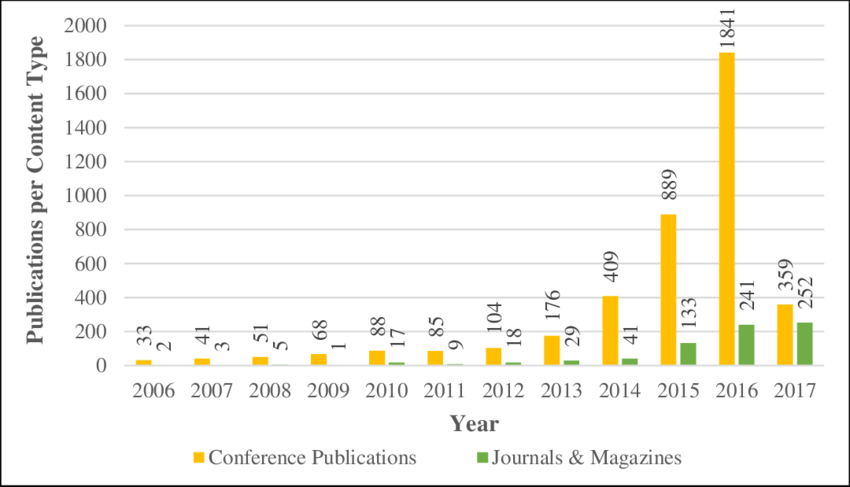
\includegraphics[scale=0.35]{pub_DL_IEEE.png}
        \caption{Publicações por ano - IEEE}    
    \end{subfigure}
    \begin{subfigure}{1\textwidth}
        \centering
        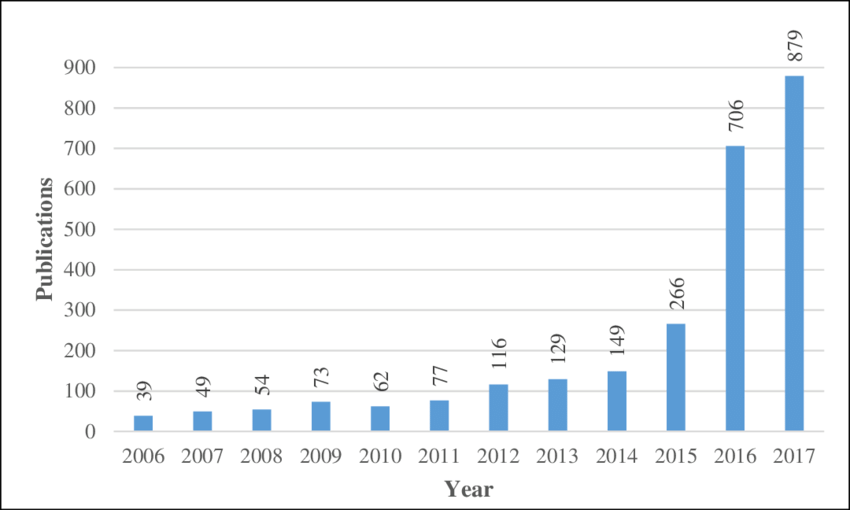
\includegraphics[scale=0.35]{pub_DL_Springer.png}
        \caption{Publicações por ano - Springer\textregistered}    
    \end{subfigure}
    \caption{Gráficos de quantidade de artigos publicados por ano relacionados com \textit{Deep Learning}}
    \label{fig:pub_DL}
\end{figure}

É possível notar um recente aumento de pesquisas relacionadas à área de aprendizado de máquina no meio científico (especialmente sobre a subdivisão de 
\textit{Deep Learning}) \cite{Study_SR_DL}. Observando a figura \ref{fig:pub_DL} \cite{Jounal_Awareness_DL} nota-se que após 2015, houve um aumento 
considerável de publicações em conferências do IEEE e o mesmo pode ser constatado para artigos em livros publicados pela editora Springer\textregistered.
Muitas dessas publicações são dedicadas para áreas de pesquisa relacionadas com áudio \cite{Study_SR_DL, Speech_proc_plus_DL, Source_Sep_DL}; de acordo com o artigo \cite{Survey_DL}, aproximadamente 20\% 
das publicações são voltadas para o tópico de reconhecimento de voz usando técnicas de \textit{Deep Learning} em suas metodologias.

% ### TODO: desafio de faltar dado para deep learning
Um dos maiores desafios enfrentados ao utilizar técnicas de \textit{Deep Learning} é de obter uma grande quantidade de dados para treinamento.
Pode-ser observar um exemplo disso em \cite{Estimation_RT_DRR,ACE_Data_Aug_Eval}, onde os autores precisaram agrupar dados de mais de 5 bases contendo
RIRs para que fosse possível treinar e avaliar suas redes.
No caso de bases de dados que envolvem RIRs, o motivo de não existir uma alta variedade de dados é devido às dificuldades
de realizar a gravação dos áudios \cite{Recording_RIR_2}.
Para gerar o impulso sonoro, é necessário de uma fonte sonora (por exemplo, um alto-falante) capaz de realizar uma varredura de senos com o mínimo de distorção
possível, ou usar um equipamento para iniciar um som de decaimento rápido e de alta intensidade (por exemplo, um balão estourando) \cite{Recording_RIR}.
A gravação do impulso requer microfones que estejam dentro de uma câmara anecoica, capacitando assim o microfone de gravar apenas o som vindo direto
da fonte sonora, e não as ondas que são refletidas nas paredes.
Não menos importante, para aumentar a quantidade de amostras na base, deve-se não só gravar o áudio não só em diferentes posições no ambiente
e distâncias da fonte-microfone, como também preparar estes mesmos procedimentos em ambientes diferentes, levando ao transporte de diversos equipamentos
especializados entre localizações físicas.

\section{\textit{Data Augmentation}}

% ### TODO: [FIGURA] explicando caminho a ser tomada

\textit{Data Augmentation} representa um conjunto de técnicas que são usadas em dados já existentes com o intuito de gerar cópias
modificadas que se enquadram para uma determinada aplicação. No contexto de \textit{Deep Learning}, essas técnicas tornam-se vitais
para incrementar artificialmente bases de dados para treinamento que não possuem uma alta variedade de amostras, e isso inclui 
dados de áudio \cite{DL_Data_Aug_sc,Metric_Data_Aug_sc}.

\begin{figure} [H]
    \centering
    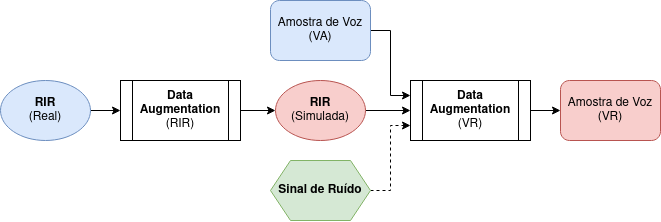
\includegraphics[scale=0.6]{flow-geral.png}
    \caption{Fluxo geral de procedimentos para gerar sinais de voz reverberantes.}
    \label{fig:flow-geral}
\end{figure} 

No escopo deste trabalho, de acordo com a figura \ref{fig:flow-geral} usaremos duas técnicas de \textit{Data Augmentation} para gerar amostras
de voz reverberantes. Uma das técnicas é voltada para simulação de RIRs, que altera suas propriedades para que possa ser simulado diferentes condições
e posições em um determinado ambiente; já a outra técnica é desenvolvida para simular ruídos no ambiente, que adiciona tanto ruídos pontuais em um trecho
da amostra de voz, sendo este convoluído com a RIR real ou simulada, quanto um ruído de fundo.

